\subsection{Pellenkoft Rulsets}

Bei der Erforschung eines Search Spaces kommen in Transformations-basierten Query Optimierern Transformationsregeln zum Einsatz. Pellenkoft et al. \cite{pellenkoft1997duplicate} \cite{manegold2000multi} \cite{pellenkoft1997complexity} stellt drei Regelsets zur Verfügung, die bei der Erzeugung eines Search Spaces zum Einsatz kommen können.

Zu Beginn besteht ein Search Space aus einem Plan. Dieser Plan stellt die Eingabe dar. Auf Ihn werden Transformationsregeln angewendet. Neue Pläne entstehen. Sollten diese Pläne noch nicht vorhanden sein, werden sie dem Suchraum hinzugefügt. Pläne auf die bereits alle anwendbaren Transformationsregeln auch angewendet wurden werden als besuchte Pläne bezeichnet. Sobald alle Pläne besucht wurden und somit auf alle Pläne Transformationsregeln angewendet wurden, ist der Suchraum vollständig erforscht und keine weiteren Pläne können gefunden werden. 

Mehrere Transformationsregeln werden gemeinsam als Regelsets bezeichnet. Pellenkoft et al. unterscheidet zwischen Regelsets, die Pläne mehrfach generieren können und Regelsets, die duplikatfrei sind. Beispielsweise kann durch die Anwendung der Regel Kommutativität auf einen Plan und erneute Anwendung auf dessen Resultat wiederum der ursprüngliche Plan generiert werden. Im Folgenden werden zwei Regelsets vorgestellt, die Duplikate bilden und ein Regelset, das duplikatsfrei ist.


\subsubsection{Regelset mit Duplikaten}

Eines der Regelsets, das zur Erzeugung eines Bushy Space genutzt werden kann, ist RS-B0. Es besteht aus drei Regeln:

\begin{itemize}
\item Kommutativität: $$ A \Join B \to B \Join A$$
\item Rechte Assoziativität: $$(A \Join B) \Join C \to A \Join (B \Join C) $$
\item Linke Assoziativität: $$A \Join (B \Join C) \to (A \Join B) \Join C$$
\end{itemize}

Das Regelset ist redundant, da mit Hilfe von Kommutativität und rechter Assoziativität. linke Assoziatvität (und vis-à-vis) erzeugt werden kann. Das daraus abgeleitete Regelset RS-B1 besteht daher aus folgenden Regeln:

\begin{itemize}
\item Swap $$ (A \Join B) \Join C \to (A \Join C) \Join B $$
\item Bottom Commutativitity $$ B_1 \Join B_2 \to B_2 \Join B_1$$
\end{itemize}

Durch die Anwendung der Regeln aus RS-B0 und RS-B1 können Pläne doppelt erzeugt werden. Am einfachsten ist dies an Hand von Kommutativität zu zeigen. Wird auf den Plan a JOIN b Kommutativität angewendet, entsteht b JOIN a, dann entsteht durch  die erneute Anwendung von Kommutativität auf den neuen Plan B JOIN A wieder der ursprüngliche Plan.

Ebenfalls können sich bei komplexeren Plänen Teilpläne gleichen. Beispielsweise enthält der Plan (A JOIN B) JOIN C den gleichen Subplan wie C JOIN (A JOIN B). Um solche Duplikate zu verhindern, wird von Pellenkoft das Prinzip der Äquivalenzklasse  angewendet.



\subsubsection{Duplikatfreie Regelsets}
Durch die Anwendung on RS-B0 bzw. RS-B1 ist es möglich, dass Varianten des Plans erneut erzeugt werden. Dieser Gefahr trägt das Regelset RS-B2 Rechnung. Es sieht vor, dass eine Regel nur genau einmal ausgeführt und andere Regeln nur einmal pro Operator ausgeführt werden dürfen. Dieses Regelset besteht aus:


\begin{itemize}
\item Kommutativität: $$ A \Join B \to B \Join A$$
\item Rechte Assoziativität: $$(A \Join B) \Join C \to A \Join (B \Join C) $$
\item Linke Assoziativität: $$A \Join (B \Join C) \to (A \Join B) \Join C$$

\item Exchange $$(A \Join B) \Join (C \Join D) \to (A \Join D) \Join (C \Join B) $$
\end{itemize}



\subsubsection{Kreuzproduktfreie Regelsets und Vollständigkeit}

Die bisherigen Regelsets können zu Kreuzprodukten führen. Ebenfalls ist nicht geklärt, ob die Regelsets vollständig sind und alle möglichen kreuzproduktfreien Bäume erzeugen. Im Folgenden wird zuerst der Begriff der Kreuzproduktfreiheit eingeführt und basierend auf diesem Begriff die Vollständigkeit erläutert.

Ein Kreuprodukt kann bei den vorliegenden Plänen dann entstehen, wenn durch die Anwendung einer Regel ein Join zwischen zwei Relationen gebildet wird, die zuvor keine Kante auf einem gegeben Join Tree hatten.

Eine Technik um kreuzproduktfreiheit bei den bisherigen Regelsets herzustellen, ist die Unterdrückung von Kreuprodukten die auch als \ac{CPS} bezeichnet wird. Der Ansatz funktioniert so, dass eine Regel, falls sie ein Kreuzprodukt erzeugt zwar als ausgeführt markiert, jedoch nicht der Baum in den Search Space aufgenommen wird. Somit werden Kreuzprodukte zwar erzeugt, aber nicht in den Suchrraum aufgenommen. Regelsets, die diese Art von Kreuzproduktunterdrückung anwenden, erhalten das Suffix CPS. Somit entstehen aus den Regelsets RS-B0, RS-B1 und RS-B2 die Regelsets RS-B0-CPS, RS-B1-CPS und RS-B2-CPS.


Eine andere wichtige Eigenschaft von Regelsets ist Vollständigkeit. Sie setzt voraus, dass Kreuzproduktfreiheit gegeben ist. Vollständigkeit liegt dann vor, wenn alle kreuzproduktfreien Pläne in einem Suchrraum erzeugt wurden.


\subsubsection{Unvollständigkeit von RS-02}


\begin{figure}[h]
  \centering
  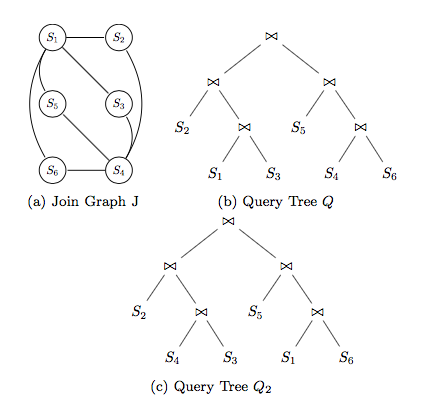
\includegraphics[width=\textwidth]{03_Related_Work/Incompleteness_RS-B2-CPS.png}
  \caption{Incompletness of RS-B2-CPS}
  \label{Incompleteness_RS-B2-CPS}
\end{figure}


\cite{shanbhag2014optimizing} stellt fest, dass RS-B0-CPS und RS-B1-CPS vollständig sind. Die Vollständigkeit von RS-B2-CPS wird jedoch in Frage gestellt und die Unvollständigkeit mit Hilfe eines Beispiels belegt. Als Beispiel dient eine Menge von Relationen, die mit Hilfe des Jointrees J (\ref{fig:Incompleteness_RS-B2-CPS}) miteinander gejoint sind. Der Initale Anfragebaum $Q1$ ist in \ref{fig:Incompleteness_RS-B2-CPS} dargestellt. Das gewünschte Ergebnis nach einer Transformation $Q2$  findet sich in \ref{fig:Incompleteness_RS-B2-CPS}. 

Bei RS-B2-CPS dürfen die Regeln R2, R3, R4 nur jeweils einmal auf einen Join-Operator angewendet werden. Keine der Regeln darf danach auf den neu generierten Operator angewendet werden. Die In \ref{fig:Q1} und \ref{fig:Q2} zeichnet sich dadurch aus, dass die Relationen $R1$ und $R4$ vertauscht sind.







\subsubsection{Vorschlag von RS-Graph}

\cite{shanbhag2014optimizing}